\chapter{One turn maze}

\section{One turn maze}
The general nature of GLGPU allowed us to explore a vast range of previously studied systems. Mills et. al. Studied vortex movements in superconducting nanowires~\cite{Mills16}. In it they performed an experiment where the vortices only felt a current in a portion of the nanowire. The vortices which were pushed by the Lorentz force then pushed against vortices which were away from the current and the whole system moved. In GLGPU, we do not have an option to make only part of the system be under the influence of a current. But what we can do is cause the vortices to have to travel in a direction perpenduclar to the one which the current would want them to by exploiting the geometry of the system. By increasing the length of the turn, we increase the "dead weight" of vortices which are being pushed by the other vortices and thereby gain a better understanding of the vortex-vortex interactions.   

\begin{figure}[htbp]
\begin{center}
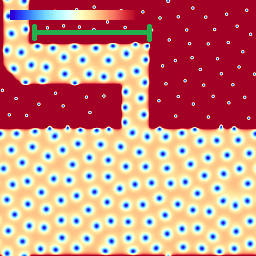
\includegraphics[scale=.50]{oneKinkDone.png}
\caption{ The amplitude of the complex order parameter. in yellow is the background superconductor, In red is the superconductor wall, and the blue dots are the vortices. In green is the parameter of interest. In this case it is the length of the "turn" which is being varied.}
\label{oneSidedY}
\end{center}
\end{figure}

\begin{figure}[htbp]
\begin{center}
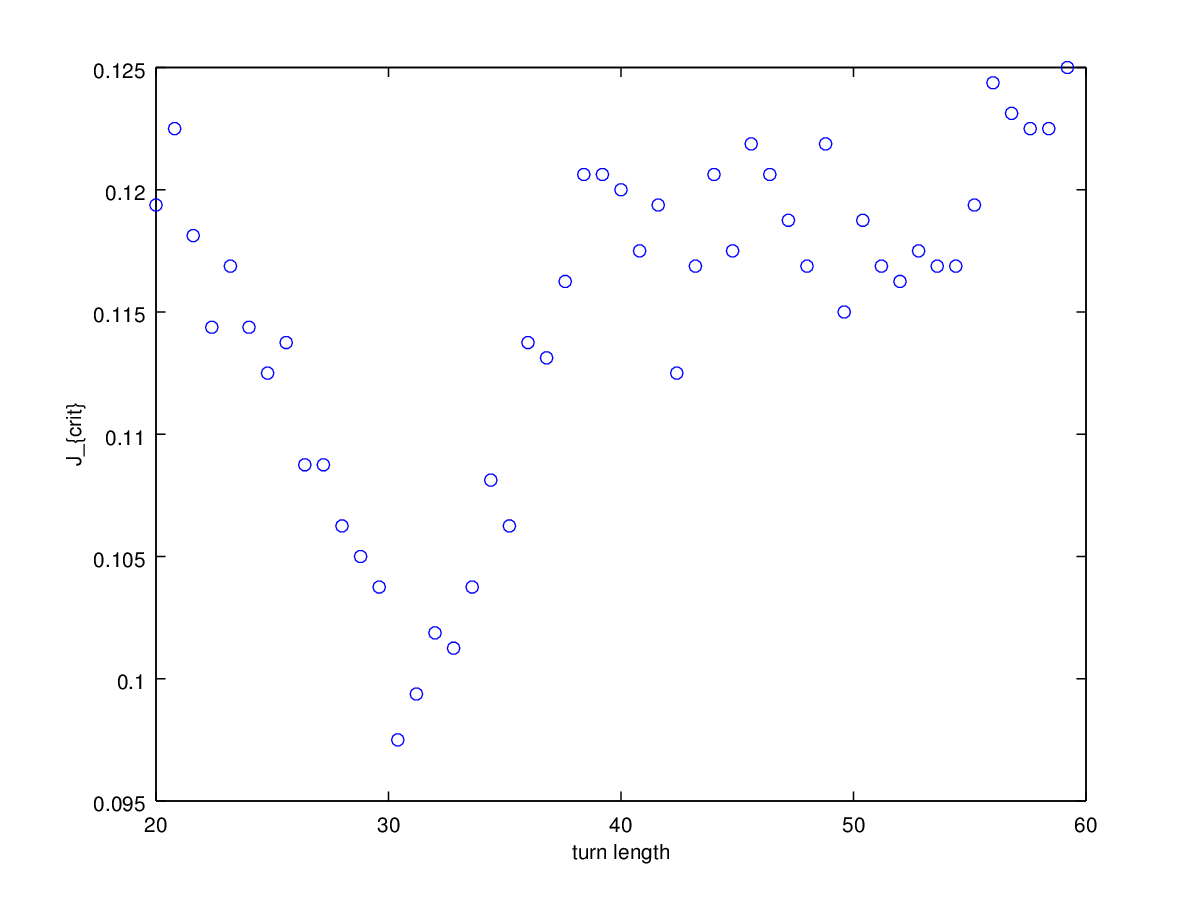
\includegraphics[scale=.50]{kinkScan.png}
\caption{ 50 values of the turn length were run in this simulation. The resulting current versus voltage information was analyzed to find the critical current .  }
\label{normalYscan}
\end{center}
\end{figure}

\section{Resistance Study}
The main purpose of our work was to try to keep the vortices from moving in the first place. But another area of research which we explored was the ability of a funneled system to slow down vortices once they had already started moving. In this study, we took the average voltage caused by vortices moving once they had depinned. Reichhardt et. al.~\cite{Reichhardt10} observed that as we increase the number of vortices, the total resistance does not change.

\begin{figure}[htbp]
\begin{center}
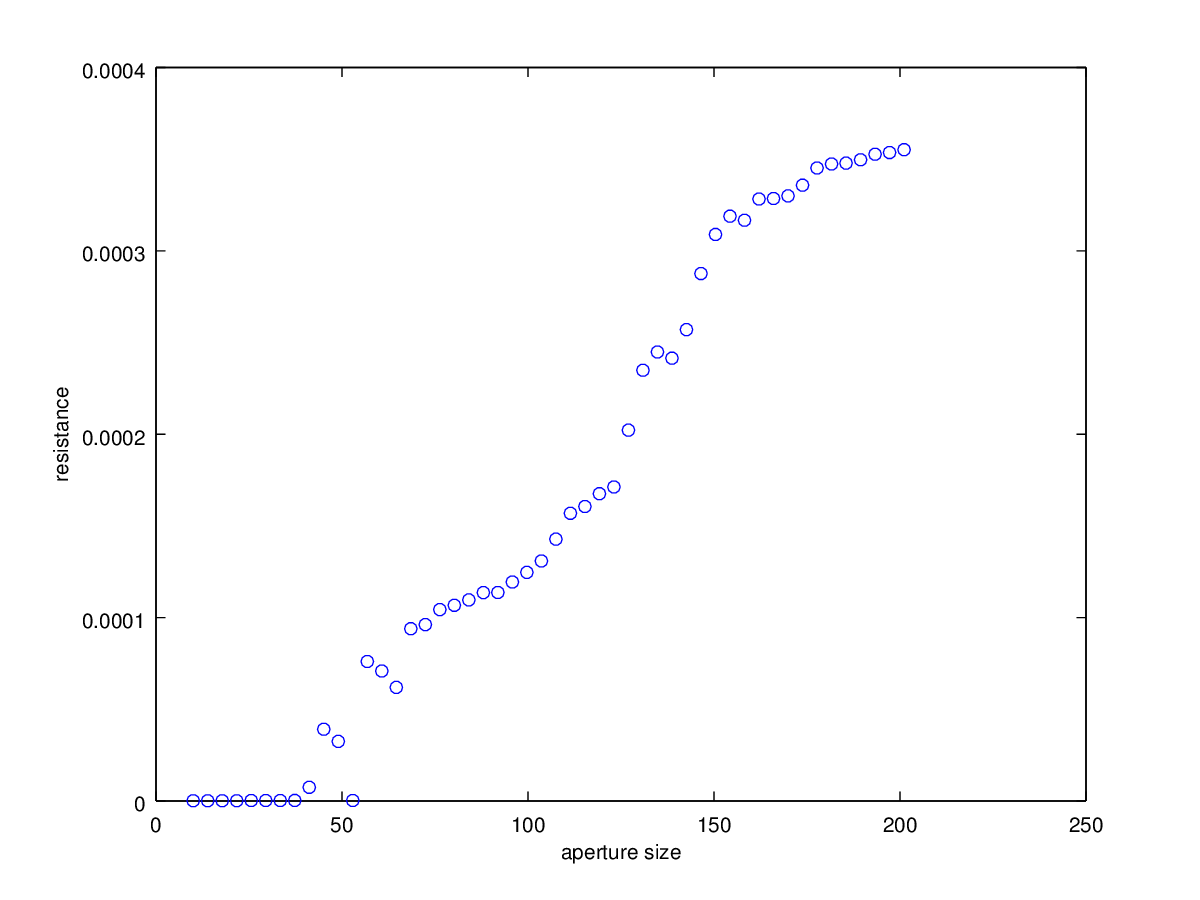
\includegraphics[scale=.50]{AvR.png}
\caption{ We can also study how the aperture size hampers vortex movement once they have already been depinned. This is a resistance plot of the constant y-position funnel. On the X axis is the size of the aperture, Y axis is the superconductive resistance. }
\label{AvR}
\end{center}
\end{figure}


